
\documentclass{article}
\usepackage{graphicx}
\usepackage{tikz}


\begin{document}


%%%%%%%%%%%%%%%%%%%%%%%%%%%%%%%%%%%%%%%%%%%%%%%%%%%%%%%%%
\definecolor{bgcolor}{rgb}{0.98, 0.98, 1.0}
\newenvironment{tikzbox}
{\begin{tikzpicture}
    \node[fill=bgcolor,rounded corners=1em,draw=black,minimum width=0.9\linewidth]}
  {;\end{tikzpicture}}

%%%%%%%%%%%%%%%%%%%%%%%%%%%%%%%%%%%%%%%%%%%%%%%%%%%%%%%%%


\begin{figure}[ht!]
  %\vspace{-1.0em}
\begin{center}
  \begin{tikzbox} {
  \begin{tikzpicture}[minimum width=0]
    \tikzstyle{label} = [node distance = 3cm,text=blue]
    \tikzstyle{mycoord} = [node distance = 0cm]
    \tikzstyle{block} = [node distance = 0.5cm,rounded corners=.00cm,
    inner sep=.1cm, fill=bgcolor, minimum height=2em,minimum width=7em]
     \node[block,name=ns1] {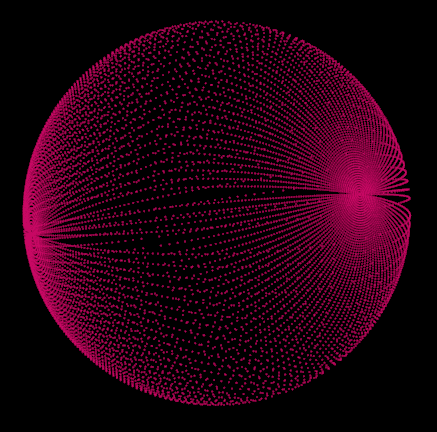
\includegraphics[width=0.25\textwidth]{./sphere_clean.png} };
     \node[block,xshift=3.5cm,name=ns2] {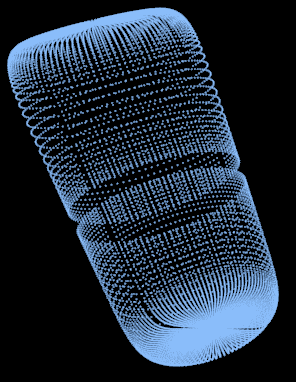
\includegraphics[width=0.25\textwidth]{./cylinder_clean.png} };
     \node[block,xshift=7cm,name=ns3] {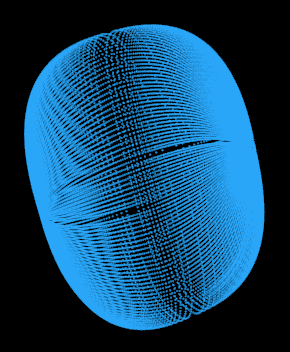
\includegraphics[width=0.25\textwidth]{./oval_clean.png} };
     \node[block,xshift=10.5cm,name=ns4] {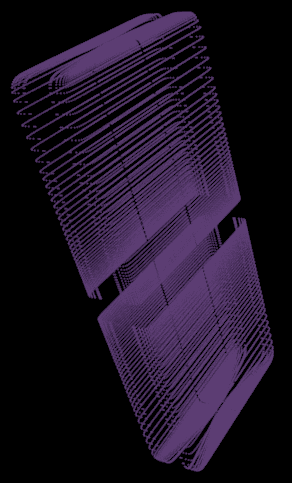
\includegraphics[width=0.25\textwidth]{./box_clean.png} };

     \node[label,below of=ns1]{Sphere};  
     \node[label,below of=ns2]{Cylinder};
     \node[label,below of=ns3]{Oval shape};
     \node[label,below of=ns4]{Box};

  \end{tikzpicture}
  }\end{tikzbox}
\caption{Clean pointcloud}
\label{fig:coverImage}
\end{center}
\vspace{-2.0em}
\end{figure}

\begin{figure}[ht!]
  %\vspace{-1.0em}
\begin{center}
  \begin{tikzbox} {
  \begin{tikzpicture}[minimum width=0]
    \tikzstyle{label} = [node distance = 3cm,text=blue]
    \tikzstyle{mycoord} = [node distance = 0cm]
    \tikzstyle{block} = [node distance = 0.5cm,rounded corners=.00cm,
    inner sep=.1cm, fill=bgcolor, minimum height=2em,minimum width=7em]
     \node[block,name=ns1] {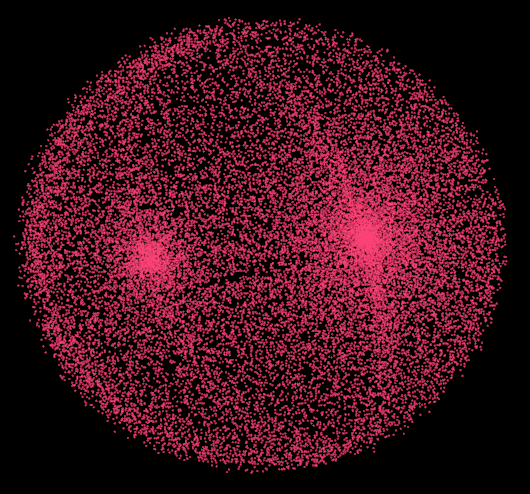
\includegraphics[width=0.25\textwidth]{./sphere_noisy.png} };
     \node[block,xshift=3.5cm,name=ns2] {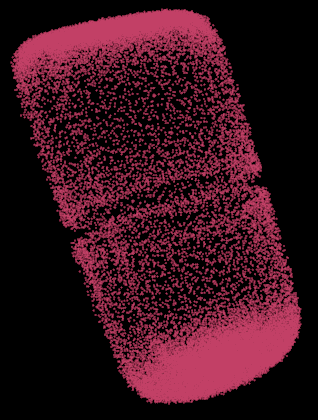
\includegraphics[width=0.25\textwidth]{./cylinder_noisy.png} };
     \node[block,xshift=7cm,name=ns3] {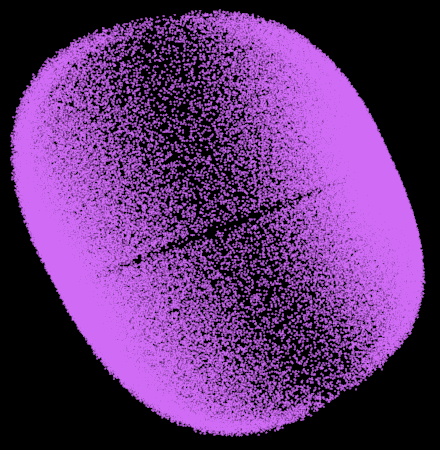
\includegraphics[width=0.25\textwidth]{./oval_noisy.png} };
     \node[block,xshift=10.5cm,name=ns4] {
\includegraphics[width=0.25\textwidth]{./box_noisy.png} };

     \node[label,below of=ns1]{Sphere};  
     \node[label,below of=ns2]{Cylinder};
     \node[label,below of=ns3]{Oval shape};
     \node[label,below of=ns4]{Box};

  \end{tikzpicture}
  }\end{tikzbox}
\caption{Noisy pointcloud}
\label{fig:coverImage}
\end{center}
\vspace{-2.0em}
\end{figure}






\end{document}